%538
\newpage
\subsection{ミニサッカーゲームで遊んでみよう}



文字とかんたんな\ruby{図形}{ず|けい}を使うだけでもゲームを作ることができます。実際にできあがっているプログラムを動かして試してみましょう。

スクリプトエディタの、ファイル→「開く」メニューから「kick.hsp」を読み込みましょう。

作業は、すべて「/home/ユーザー名/04」フォルダで行ないます。

見つからない場合は、まわりの友達か、近くの先生に聞いてみてください。



[F5]キーで実行すると、ミニサッカーゲームが動きます。



\begin{figure}[H]
    \begin{center}
      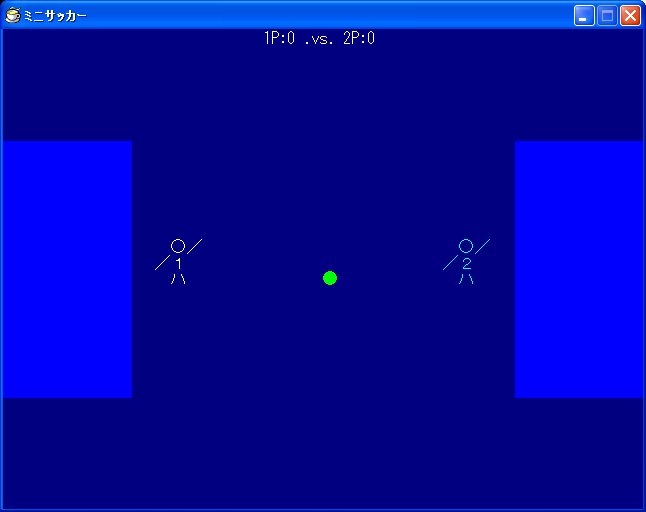
\includegraphics[keepaspectratio,width=9.075cm,height=7.197cm]{text04-img/text04-img005.png}
      \caption{ミニサッカーゲームの画面}
    \end{center}
    \label{fig:prog_menu}
\end{figure}


このゲームは二人で\ruby{対戦}{たい|せん}します。

\ruby{隣}{となり}の席にいる人と、2人1組になって\ruby{一緒}{いっ|しょ}に遊んでみてください。

左側の「1」の人をキーボードの左側で\ruby{操作}{そう|さ}します。




\ \ \ \ [W]

[A] \ \ \ \ [D] \ \ \ \ [S] = ゴール前にもどる

\ \ \ \ [X]



右側の「2」の人をキーボードの右側で操作します。




\ \ \ \ [↑]

[←] \ \ \ [→] \ \ \ \ [Enter] = ゴール前にもどる

\ \ \ \ [↓]




それぞれのプレイヤーは足でボールを蹴って遠くに飛ばすことができます。

\ \ \ \ 「1」の人は右のゴールへ、

\ \ \ \ 「2」の人は左のゴールへボールを入れたら点が入ります。


\ \ \ \ 3点先に取った人の勝ちです。

\ \ \ \ 同じグループの友達と対戦してみましょう。



\begin{figure}[H]
    \begin{center}
      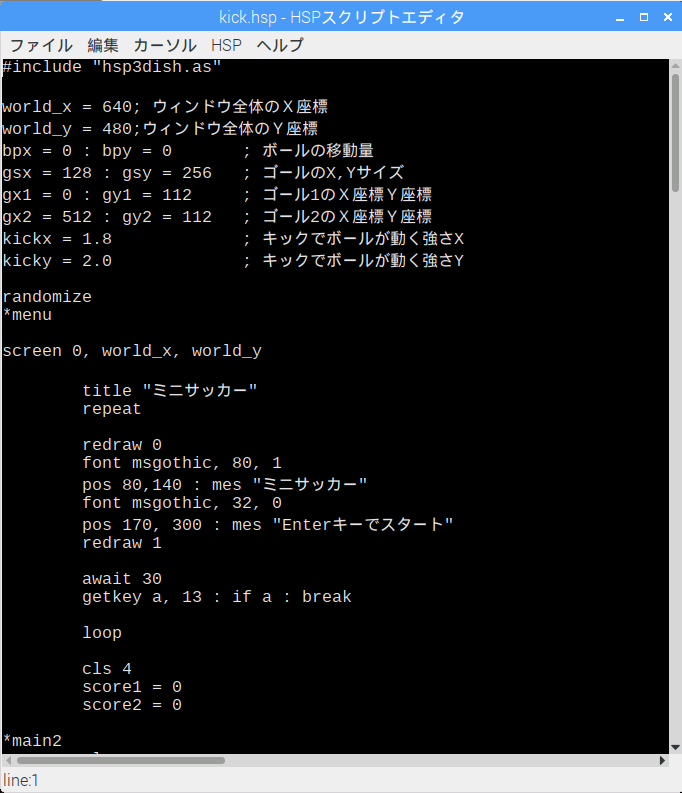
\includegraphics[keepaspectratio,width=9.657cm,height=11.229cm]{text04-img/text04-img006.png}
      \caption{ミニサッカーゲームのプログラム}
    \end{center}
    \label{fig:prog_menu}
\end{figure}


\newpage
\subsection{例題に挑戦しよう}

終わってしまった人は、以下の例題にも挑戦してみよう。


・ミニサッカーゲームの人を改造する

・ミニサッカーゲームのボールや色を変える

・ミニサッカーゲームの動きを改造する



例題の考え方がわからない時は、近くのTAか先生に聞いてください。

わからない所は、そのままにせず、必ず答えを見つけてから先に進みましょう。


